\textbf{COLUNI 2022 -- Questão 34}\par\medskip Observe o esquema sobre o fenômeno transição demográfica.

% COLUNI-AUTO-FIGURES-BEGIN
\begin{figure}[htbp]
\centering
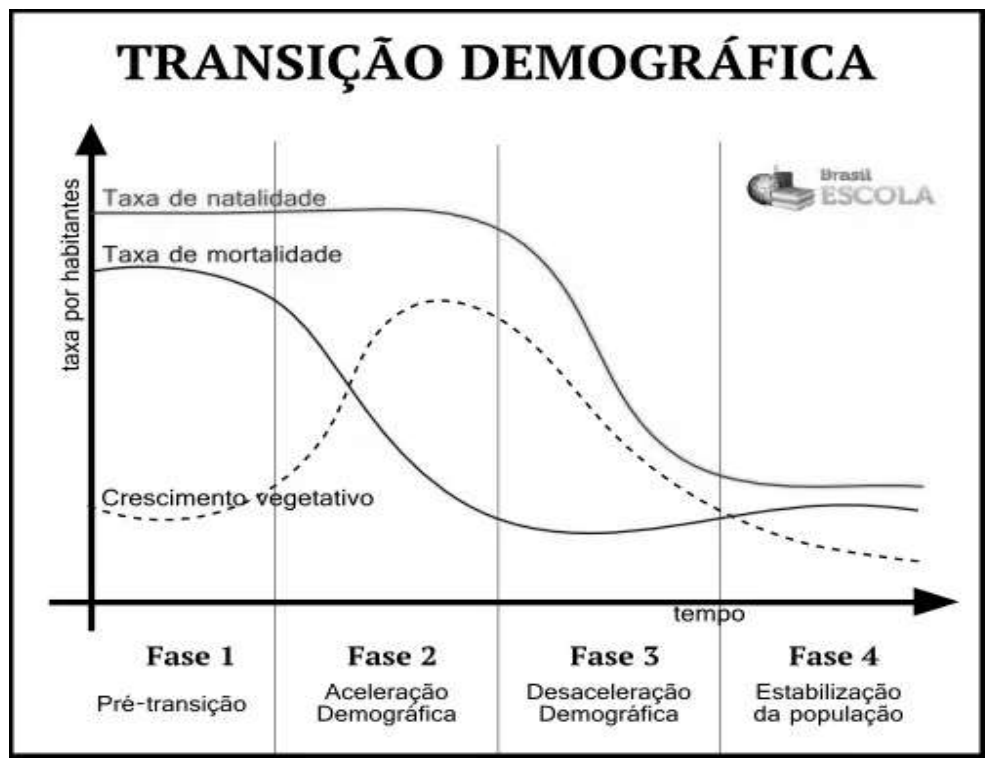
\includegraphics[width=0.95\linewidth]{static/simulados/coluni/figuras/2022/questao-34/figura-1.png}
\end{figure}
% COLUNI-AUTO-FIGURES-END

Disponível em: https://brasilescola.uol.com.br/geografia/transicao-demografica.htm. Acesso em: 15 fev. 2020.

\par

O fenômeno da transição demográfica relaciona as variações entre as taxas de mortalidade e de natalidade em uma dada sociedade representada no esquema. Sobre esse fenômeno, é CORRETO afirmar que:


\begin{enumerate}
\item na fase 4, as taxas de mortalidade e de natalidade encontram-se baixas, com crescimento natural baixo e
      com aumento da população de idosos.
\item na fase 2, a saúde da população começa a melhorar lentamente, porém a taxa de mortalidade permanece
      elevada.
\item na fase 3, com a urbanização, as taxas de mortalidade e de natalidade são reduzidas, tornando o país
      desenvolvido social e economicamente.
\item na fase 1, a pirâmide populacional é ampla na base, mantém-se larga em direção ao topo, com altas taxas
      de mortalidade infantil.
\end{enumerate}
